\documentclass{article}
\usepackage[utf8]{inputenc}
\usepackage[spanish]{babel}
\usepackage{amsmath}
\usepackage{xcolor}



\begin{document}

\title{Respuestas en LaTeX}
\author{}
\date{}

\maketitle

\documentclass{article}
\usepackage[utf8]{inputenc}
\usepackage[spanish]{babel}

\begin{document}

\begin{titlepage}
    \centering
    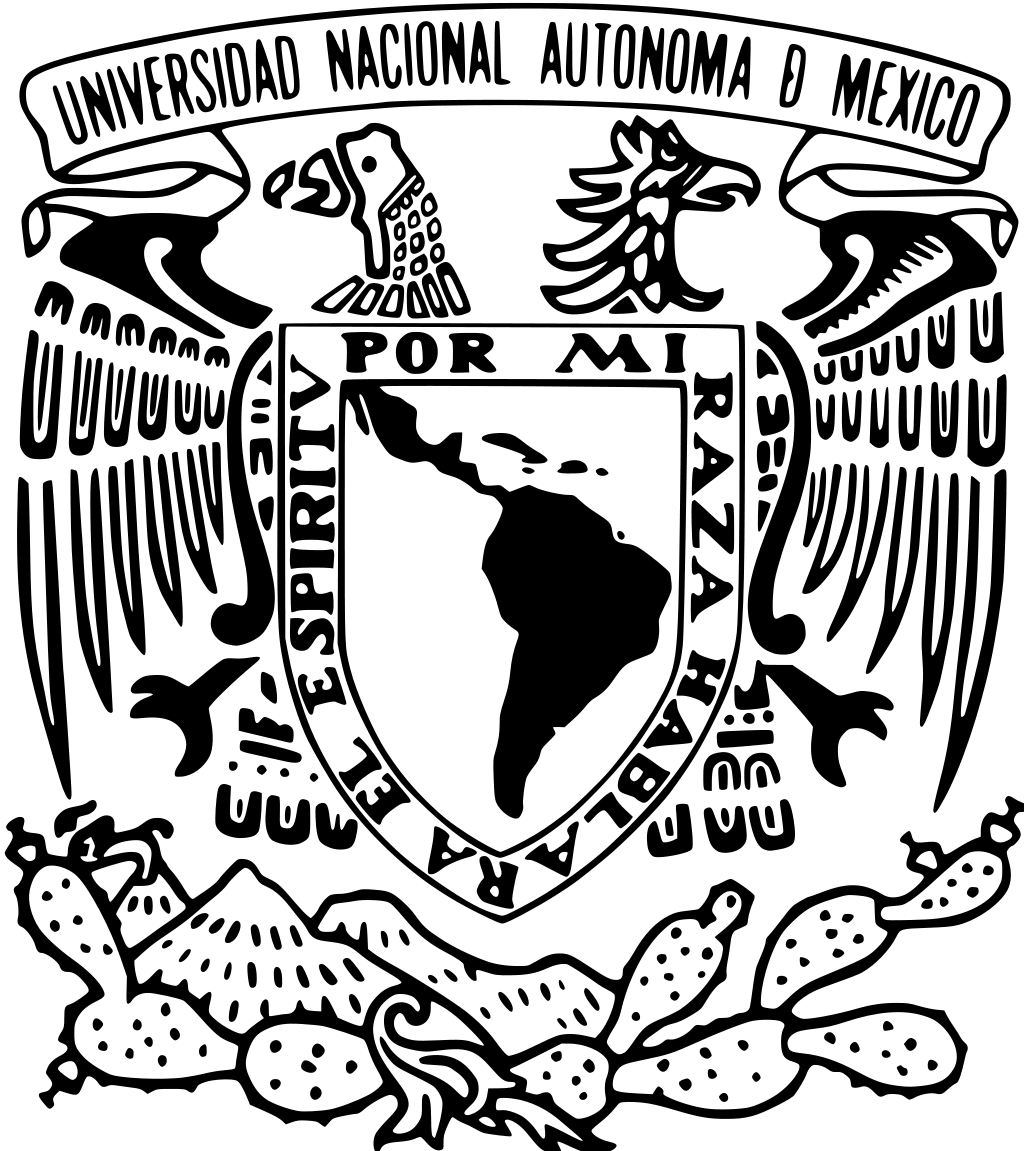
\includegraphics[width=0.4\textwidth]{unam_logo.png}\par\vspace{1cm}
    {\scshape\Large Universidad Nacional Autónoma de México \par}
    \vspace{1cm}
    {\scshape\Large Facultad de Ingeniería \par}
    \vspace{1.5cm}
    {\huge\bfseries Arquitectura de Computadoras \par}
    \vspace{2cm}
    {\Large\itshape David Rivera Morales\par}
    \vfill
    {\large \today\par}
\end{titlepage}

\end{document}



\section*{Respuestas}

\begin{enumerate}
    \item Expresar -31 y +31 en 8 bits en el sistema de complemento a 1:
    \begin{itemize}
        \item +31 en binario: \textit{0001 1111}
        \item Para obtener -31 en complemento a 1, invertimos todos los bits de +31, resultando en \textit{1110 0000}.
    \end{itemize}
    
    \item Expresar +13 y -13 en 8 bits en el sistema de complemento a 2:
    \begin{itemize}
        \item +13 en binario: \textit{0000 1101}
        \item Para obtener -13 en complemento a 2, primero invertimos todos los bits de +13 para obtener \textit{1111 0010} y luego sumamos 1, resultando en \textit{1111 0011}.
    \end{itemize}
    
    \item Rango de números representables en complemento a dos con 4 bits: \textit{-8 a +7}.
    
    \item El número \((10110101)_2\) en base decimal: Para convertir a decimal, consideramos el primer bit como el signo (1 indica negativo en complemento a 2), invertimos los bits para obtener \(01001010\), sumamos 1 para recuperar el valor absoluto, \(01001011\), que es 75 en decimal. Por lo tanto, el número es \textit{-75}.
    
    \item El número \((00110111)_2\) en base decimal: Para convertir directamente a decimal, calculamos \(2^5 + 2^4 + 2^2 + 2^1 + 2^0 = 55\). \textit{55}.
    
    \item Cuatro unidades funcionales principales de una computadora:
    \begin{enumerate}
        \item Unidad de Control (UC): Dirige el funcionamiento de la CPU.
        \item Unidad Aritmético-Lógica (ALU): Realiza operaciones aritméticas y lógicas.
        \item Memoria: Almacena datos e instrucciones.
        \item Dispositivos de Entrada/Salida: Comunicación con el exterior.
    \end{enumerate}
    
    \item Operación \(-3 - 6\) en binario con 4 bits: \(-3\) es \(1101\) y \(-6\) es \(1010\) en complemento a 2. La suma resulta en \(1001\), que representa \textit{-7} debido a desbordamiento.
    
    \item Operación \(9 + 3\) en binario con 4 bits: \(9\) es \(1001\) y \(3\) es \(0011\) en binario. La suma resulta en \(1100\), que representa \textit{12} en decimal.
    
    \item Suma de 2 bits \(01 + 11 = 100\), con desbordamiento, el resultado sería \(00\) con un bit de acarreo (\(1\)).
    
    \item Suma los siguientes dos números \((10011011)_2 + (11101100)_2\). Explica qué sucede con el acarreo. La suma es \(110000111\). El acarreo en el bit más significativo indica un desbordamiento para representaciones de 8 bits, mostrando que el resultado excede el rango representable en 8 bits.
    
    \item Representa el número 39,1 en base 2 usando el estándar IEEE 754. Para representar 39,1 en IEEE 754, convertimos primero la parte entera a binario, que es \(100111\), y luego la parte fraccionaria. La parte fraccionaria se convierte multiplicando sucesivamente por 2 y tomando la parte entera del resultado hasta obtener un patrón repetitivo o cero. Este proceso se ajusta al formato de punto flotante IEEE 754, considerando el signo, el exponente ajustado y la mantisa.
    
    \item Representa el número 576,65 en base 2 usando el estándar IEEE 754. Similar al procedimiento anterior, convertimos la parte entera \(576\) a binario y seguimos un proceso para convertir la parte fraccionaria \(0,65\) a binario. Luego, ajustamos el número al formato IEEE 754.
    
    \item ¿Qué ventajas y desventajas puedes encontrar en el modelo de la arquitectura de Von Neumann? Ventajas: Simplicidad en diseño e implementación. Desventajas: El cuello de botella del bus de datos debido a la arquitectura de programa almacenado.
    
    \item La Arquitectura Von Neumann fue descrita por el matemático y físico John von Neumann y otros, en el primer borrador de un informe sobre el EDVAC. ¿Qué cambios aprecias hoy en día en tu computador que no se ven descritos por el diagrama dado en 1945? Hoy en día, las computadoras incluyen múltiples núcleos de CPU, gráficos integrados, y arquitecturas de memoria avanzadas que van más allá de la simplicidad del modelo original de Von Neumann.
\end{enumerate}

\end{document}
